\section{Hardware struktur og funktionalitet}
Til mikroprocessoren er tilsluttet to sensorer, der hver måler en forskellig temperatur. Den ene er sat direkte på vandledningen, og måler temperaturen på røret, mens den anden sensor sidder så den kan måle temperaturen og luftfugtigheden i rummet - ca. 10 cm fra røret.\newline
Microprocessoren tilspørger sensorerne samtidig og får begge temperaturer samt luftfugtigheden i rummet, og sender disse data til en modtager, en gang hvert 10. sekund.\newline
Serveren eller computeren der modtager data står herefter for udregningen af forskellen på temperaturerne og, ud fra denne, tegning af graf eller visning af data som tekst i terminalen.
\\\\

\fxnote{beskriv diagrammet og giv et overblik over hardware strukturen}

\begin{figure}[h!]
  \caption{fase1.}
  \centering
  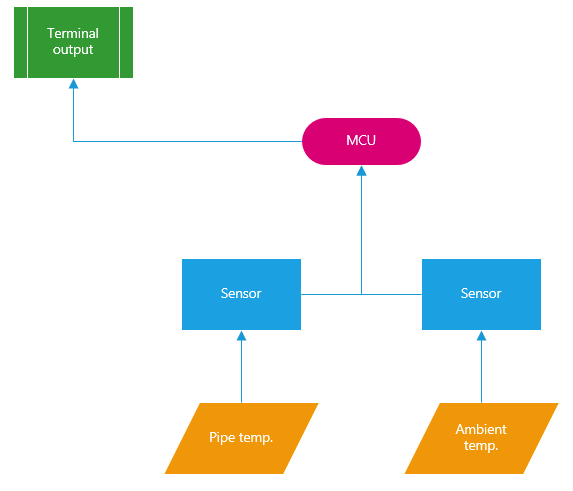
\includegraphics[width=0.5\textwidth]{figures/Phase1.PNG}
\end{figure}


\fxnote{skriv afsnit om mikroprocessoren, nævn hvorfor vi ikke bruger UCN board}




\fxnote{Indsæt undersektioner med de forskellige komponenter  og beskriv disse}
